\cleardoublepage

\chapter{Exploración del modelo predictivo}
\label{makereference4}

\section{Introducción a los modelos predictivos}
\label{makereference4.1}

%TODO HACER ESTO, PERO BIEN MAJA
 ``Cada día la gente se enfrenta a preguntas como: ¿Qué ruta debo tomar? ¿Debo cambiar de compañía telefónica? ¿Debo invertir mi dinero?
 
Lo que se quiere es conocer eventos futuros y sobre todo, conocerlos lo mejor posible.

La mayor parte de las veces se toma decisiones basándonos en información, pero muchas otras nos guiamos por nuestra intuición o la propia experiencia.

Pero de todas maneras se está prediciendo a partir de la información y experiencia que tenemos y tomando decisiones a partir de estas predicciones. '' 


Cuando hablamos de modelos predictivos nos estamos refiriendo al análisis que agrupa una serie de técnicas para conseguir analizar datos reales tanto actuales como históricos y así conseguir predicciones. Con esta predicción podremos saber cuanto se acerca nuestra predicción a la realidad.

\section{Descripción de las librerías usadas}
\label{makereference4.2}
	\subsection{Scikit-learn}
	\label{makereference4.2.1}
	Scikit-learn es una biblioteca de aprendizaje de software libre para el lenguaje de programación Python. Cuenta con varios algoritmos de clasificación, regresión y agrupación, incluyendo máquinas de vector de apoyo, bosques aleatorios, aumento de gradiente, k-medios y DBSCAN, y está diseñado para interoperar con las bibliotecas numéricas y científicas Python NumPy y SciPy. (\cite{ARP:Scikit:2017})
	
	\subsection{NumPy}
	\label{makereference4.2.2}
	NumPy es una extensión de Python, que le agrega mayor soporte para vectores y matrices, constituyendo una biblioteca de funciones matemáticas de alto nivel para operar con esos vectores o matrices. (\cite{ARP:Numpy:2017})
	
	\subsection{SciPy}
	\label{makereference4.2.3}
	SciPy es una biblioteca open source de herramientas y algoritmos matemáticos para Python. SciPy contiene módulos para optimización, álgebra lineal, integración, interpolación, funciones especiales, FFT, procesamiento de señales y de imagen, resolución de ODEs y otras tareas para la ciencia e ingeniería. (\cite{ARP:Scipy:2017})
	
\section{Algoritmos utilizados}
\label{makereference4.3}
	\subsection{Regresión Lineal}
	\label{makereference4.3.1}

	La \textbf{regresión lineal} es un modelo matemático que trata de hallar los coeficientes de una \textbf{combinación lineal} que mejor se ajusten a un conjunto de puntos dispersos conocidos a través del método de los \textbf{mínimos cuadrados}. Esto es, trazar una línea en el espacio que pase lo más próximo posible a todos los puntos.

	Al conocer dicha función lineal, podremos \textbf{``predecir''} con cierto grado de exactitud, lo que pasará.

	\begin{figure}[htb]
		
		\begin{center}
			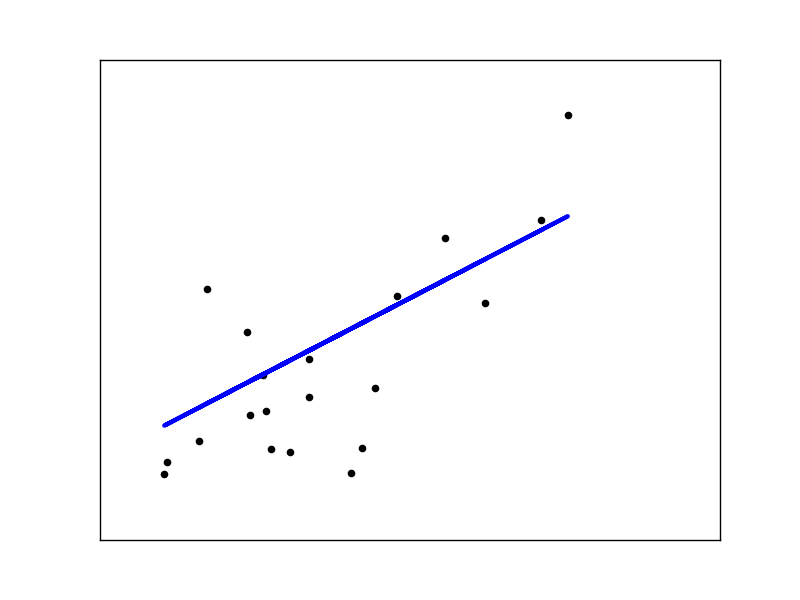
\includegraphics[height=3.5in]{figures/regression.png}
			\caption{Regresión lineal [Fuente: \href{www.wikipedia.org}{Wikipedia}]}
		\end{center}
		
		\label{regression}
	\end{figure}
	
	La recta que se puede ver en la gráfica \ref{regression}, muestra cómo la \textbf{regresión lineal} intenta dibujar una línea que minimice mejor la suma residual de cuadrados entre las respuestas observadas en el conjunto de datos, y las respuestas predichas por la aproximación lineal.
	También se calculan los coeficientes, la suma residual de cuadrados y el puntaje de varianza.

	\subsection{SVR (Support Vector Regression)}
	\label{makereference4.3.2}

	SRV es una nueva versión de SVM para regresión. SVM es un algoritmo de aprendizaje supervisado de la familia de los \textbf{clasificadores}.

	El término \textbf{clasificador} se utiliza en referencia al algoritmo utilizado para asignar un elemento entrante no etiquetado en una categoría concreta conocida. Dicho algoritmo, permite pues, ordenar o disponer por clases elementos entrantes, a partir de cierta información característica de estos.

	En SVM los datos son etiquetados en distintas clases y el clasificador intentará construir un hiperplano o conjunto de hiperplanos dentro del conjunto de datos que mejor separe las clases unas de otras. Ver figura \ref{svm}.

	\begin{figure}[htb]
		
		\begin{center}
			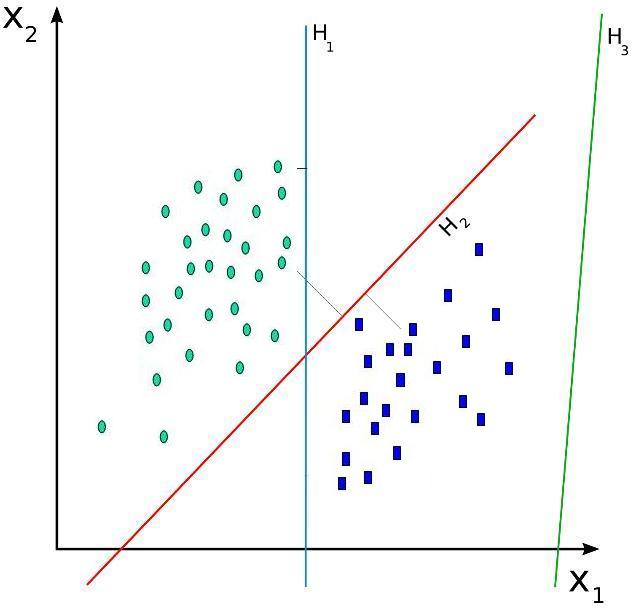
\includegraphics[height=3.5in]{figures/svm.jpg}
			\caption{SVM [Fuente: \href{www.wikipedia.org}{Wikipedia}]}
		\end{center}
		\label{svm}
	\end{figure}

	Las características más notables de los clasificadores SVM son:
	\begin{itemize}
		\item Proyectar previamente los datos a un espacio de dimensionalidad superior.
		\item Buscar el hiperplano que tenga la máxima distancia con los puntos que estén más cerca de él mismo. Es decir, que dejen una mayor margen entre los datos.
	\end{itemize}

	La diferencia entre SVR y SVM es que SVR intenta hacer una regresión a partir de el clasificador. Para esto, realiza un mapeo no lineal de los datos del entrenamiento a un espacio de mayor dimensión, donde podremos realizar una regresión lineal. Ver figura \ref{svr}.

	\begin{figure}[htb]
		\begin{center}
			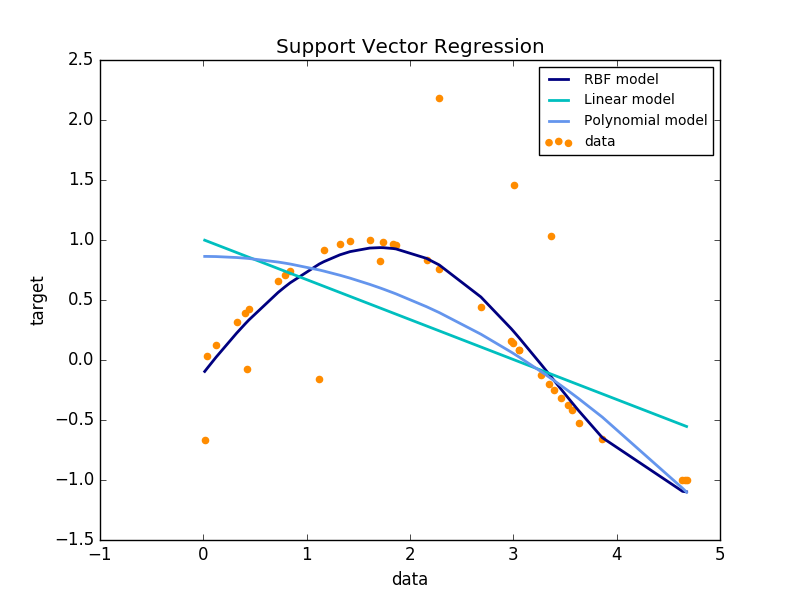
\includegraphics[height=3.5in]{figures/svr.png}
			\caption{SVR [Fuente: \href{http://scikit-learn.org/stable/auto_examples/svm/plot_svm_regression.html}{scikit learn}] }
		\end{center}
		\label{svr}
	\end{figure}
	
	\subsection{Redes Neuronales}
	\label{makereference4.3.3}
	Las redes neuronales son un algoritmo de aprendizaje supervisado de la familia de los \textbf{clasificadores}, al igual que SVR \ref{makereference4.3.2}.

	Se basan en el principio del funcionamiento de las neuronas del cuerpo humano. Cada neurona recibe varias señales y propaga, en función de estas, otro resultado al resto de la red.

	Las neuronas de estas redes, son llamadas \textbf{perceptrones}. Son unidades funcionales sin una función específica que buscan aplicar un peso a las señales recibidas y en base a ello, envía un señal a otra neurona.

	\begin{figure}[htb]
		\begin{center}
			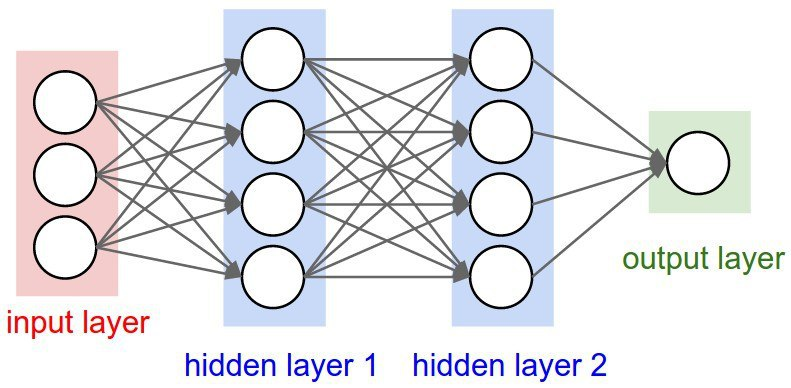
\includegraphics[width=4.5in]{figures/neural_network.jpg}
			\caption{Red neuronal [Fuente: \href{www.scikit-learn.org}{scikit-learn}]}
		\end{center}
		\label{network}
	\end{figure}

	La distribución de las neuronas se realiza en distintas capas. La primera capa ``capa de entrada'' recibe los datos de entrada. La última capa proporciona los resultados de la \textbf{clasificación}, normalmente la clase a la que pertenecen los datos de entrada.

	Las capas intermedias buscan aumentar la posibilidad de ajuste de los pesos. El ajuste de estos pesos se realiza de la siguiente forma:

	\begin{itemize}
		\item Cada neurona empieza con unos pesos aleatorios.
		\item Se introducen datos aleatorio dentro del conjunto total de entrada.
		\item La red genera un vector de datos de salida.
		\item Esta salida se compara con el resultado esperado.
		\item El \textbf{error} obtenido se propaga a la capa de neuronas anterior (\textbf{back-propagation}) y se usa para ajustar los pesos.
		\item Se continua propagando el error hacia atrás ajustando los pesos de cada capa hasta alcanzar la \textbf{capa de entrada}.
		\item Esto se repetirá con diferentes datos de entrenamiento.
 	\end{itemize}

	Es tarea del desarrollador la elección del número de capas y de neuronas en cada capa.

\section{Método del estudio}
\label{makereference4.4}
	\subsection{Grid Search}

	\begin{figure}[htb]
		\begin{center}
			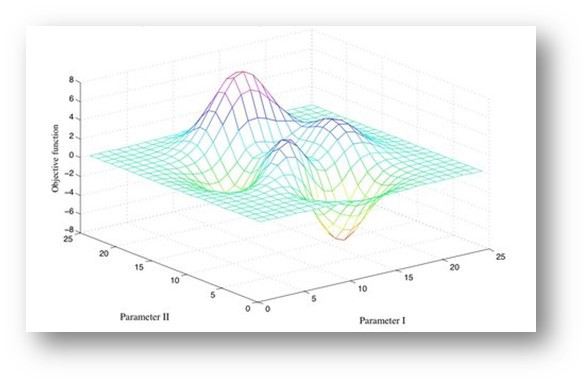
\includegraphics[width=4.5in]{figures/grid_search.jpeg}
			\caption{Grid Search [Fuente: \href{www.scikit-learn.org}{scikit-learn}]}
		\end{center}
		\label{grid}
	\end{figure}

	Para optimizar la elección del modelo predictivo y sus parámetros, necesitamos estudiar el comportamiento que tiene un modelo con todos sus posibles parámetros teniendo así la certeza de que elegimos la mejor configuración.

	Esta es una tarea que no se puede llevar a cabo, por lo que existen distintas maneras de abordar el problema. En respuesta a esto, surgen métodos de análisis más optimos, entre ellos encontramos \textbf{Grid Search}.

	\textbf{Grid Search} es un método de estudio ya implementado al que se le expecifica los algoritmos a estudiar y rangos para los distintos parámetros de cada uno. 

	Este método observa qué muestra del rango es la que obtiene un ``mejor resultado'' y vuelve a realizar el estudio ``haciendo zoom'' con centro en esta muestra.

	\begin{figure}[htb]
		\begin{center}
			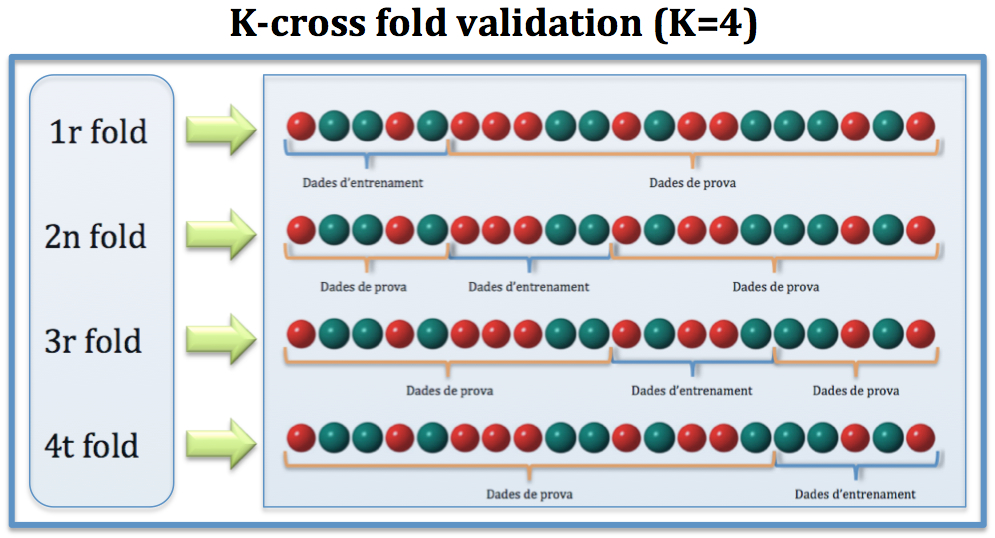
\includegraphics[width=4.5in]{figures/Cross-Validation.jpg}
			\caption{Validación cruzada [Fuente: \href{www.scikit-learn.org}{scikit-learn}]}
		\end{center}
		\label{cross}
	\end{figure}

	Para calcular el mejor resultado se utiliza una técnica llamada ``K-Fold Cross-Validation''. Esta técnica divide los datos en ``k'' conjuntos. Uno de ellos es utilizado como datos de prueba y el resto como datos de entrenamiento. Se realiza un proceso de validación y se repite k veces con cada uno de los posibles subconjuntos.

	Al realizar este proceso de validación con datos conocidos, puede conocer la precisión o ``accuracy'' que es capaz de obtener un modelo predictivo.

	Una vez realizado el estudio con los distintos modelos y parámetros se puede observar cual es la mejor configuración para nuestros datos.
	
	Existen otros métodos de exploración del modelo predictivo como por ejemplo \textbf{Randomized Parameter Optimization}, que realiza el estudio probando con configuraciones aleatorias.

	\subsection{Sistema de entrenamiento}
	%TODO Referenciar SCIKIT
	Para llevar a cabo la implementación de Grid Search, hemos utilizado las funciones proporcionadas por \textbf{scikit-learn}.
	Esta librería ofrece una implementación de Grid Search a través de una función que nos permite abstraer el algoritmo de los modelos predictivos.

	%TODO Añadir JSON tunned parameters
	%TODO Referenciar JSON
	Hemos desarrollado distintas baterías de prueba a través de ficheros en formato \textbf{JSON} que definen los distintos modelos y parametros que debe explorar Grid Search.
	Estas baterias de prueba son procesadas por un algoritmo encargado de instanciar los distintos modelos y suministrárselos a Grid Search.
	Los resultados obtenidos de cada prueba son almacenados en archivos con formato CSV para su posterior análisis.
	%TODO Añadir foto CSV resultados
	%TODO Describir archivos con parametros ajustados del modelo elegido

\section{Modelo escogido}
\label{makereference4.5}
%TODO explicar el modelo elegido